\documentclass[10pt,a4paper]{article}
\usepackage[utf8]{inputenc}
\usepackage{amsmath}
\usepackage{amsfonts}
\usepackage{amssymb}
\usepackage[]{algorithm2e}
\usepackage{graphicx}
\usepackage[left=2cm,right=2cm,top=2cm,bottom=2cm]{geometry}

\begin{document}

\title{LINGI2261: Artificial Intelligence \\
Assignement 3 : Adversarial Search}
\author{Group 8: Ndizera Eddy \and El Jilali Solaiman}
\date{\today}
\maketitle

\section{Alpha-Beta search}

\subsection{Perform the MiniMax algorithm on the tree in Figure 1, i.e. put a value to each node. Circle the move the root player should do.}

\begin{figure}[h]
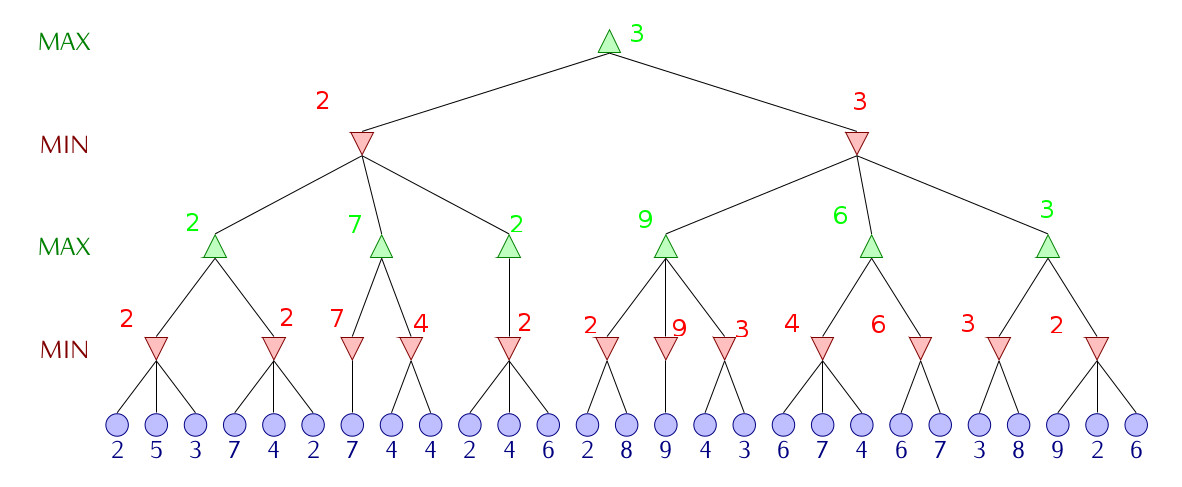
\includegraphics[scale=0.4]{img/minimax.jpg} 
\caption{\label{minimax} MiniMax}
\end{figure}

\subsection{Perform the Alpha-Beta algorithm on the tree in Figure 2. At each non terminal node, put the successive values of $ \alpha $ and $ \beta $. Cross out the arcs reaching non visited nodes. Assume a left-to-right node expansion.}

\begin{figure}[h]
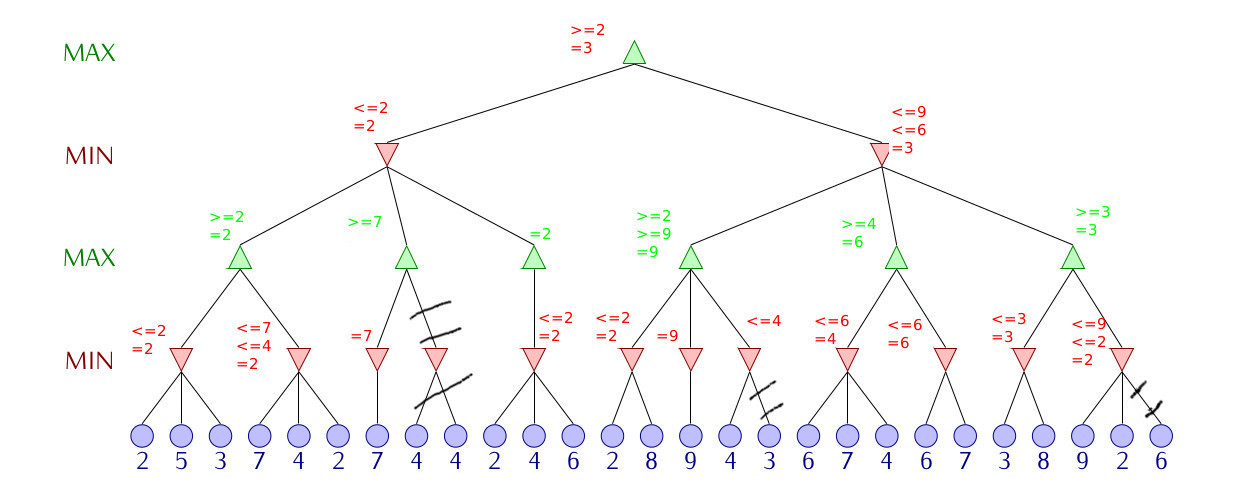
\includegraphics[scale=0.4]{img/alphabeta_left.jpg} 
\caption{\label{alphabetaleft} Alpha-Beta, left-to-right expansion}
\end{figure}

\subsection{Do the same, assuming a right-to-left node expansion instead (Figure 3).}

\begin{figure}[h]
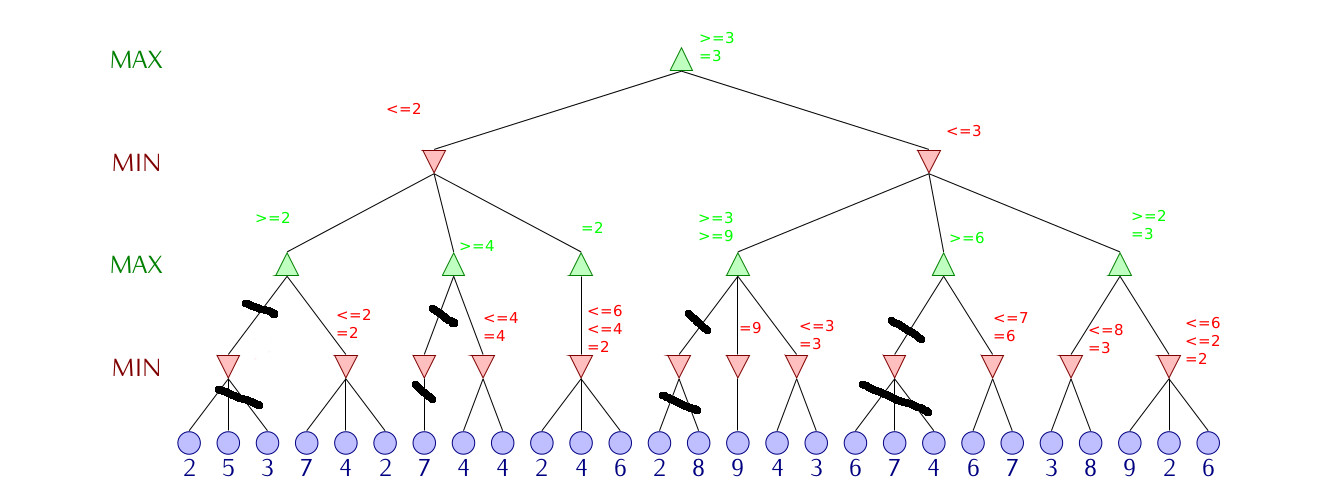
\includegraphics[scale=0.4]{img/alphabeta_right.jpg} 
\caption{\label{alphabetaright} Alpha-Beta, right-to-left expansion}
\end{figure}

\subsection{Can the nodes be ordered in such a way that Alpha-Beta pruning can cut off more branches (in a left-to right node expansion)? If no, explain why; if yes, give the new ordering and the resulting new pruning.}

Yes, if we order the nodes in increasing order like shown in Figure \ref{alphabetanodes}, the Alpha-Beta pruning will cut off more branches. The nodes must be set in that order because it's MIN that chooses the action to pick in the bottom of the tree.
The idea is to first examine the best node at each depth (Min or Max) \\
\begin{itemize}
	\item For max nodes, we want to visit the best child (>=) first so that time is not wasted in the rest of the children exploring worse scenarios.
	\item For min nodes, we want to visit the worst child first
\end{itemize}
If we reorder all the tree in that way, we can pass more childrens nodes because at the parent level all those childrens nodes will imply a cutoff.


\begin{figure}[h]
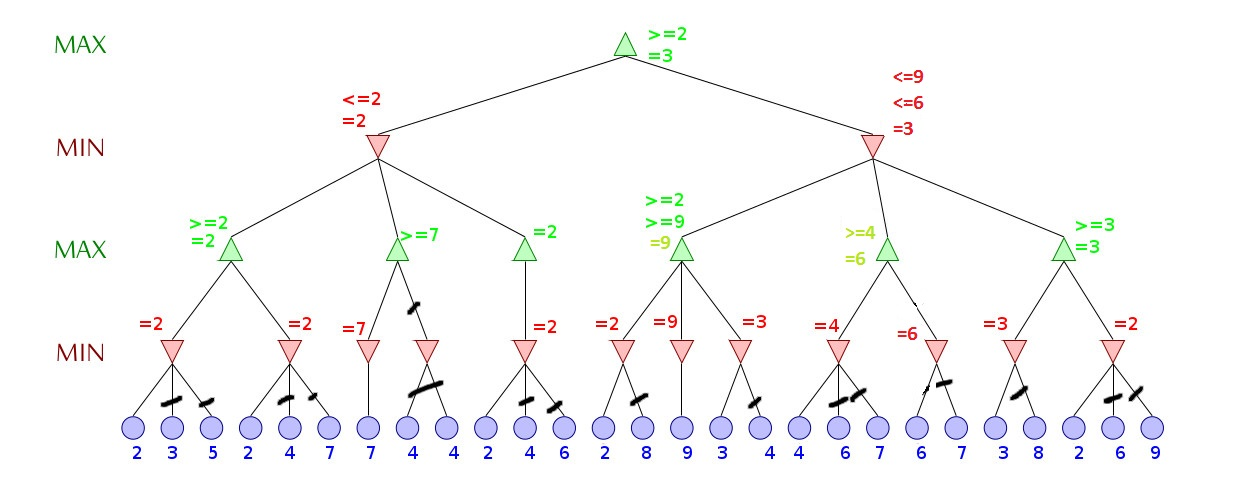
\includegraphics[scale=0.4]{img/alphabeta_nodes.jpg} 
\caption{\label{alphabetanodes} Alpha-Beta, left-to-right expansion}
\end{figure}

\section{Avalam}

\subsection{A basic Alpha-Beta Agent}

The basic Alpha-Beta Agent can be found on INGInious.

\subsection{Comparison of two evalutaion functions}

\subsubsection{Launch a game where one of the agents is the basic agent described before against another agent where the basic evaluate method has been replaced such that it returns directly the result of Board.get\_score instead of -1, 0 or 1. Watch the replay of the match. What do you observe? Does one of the agent clearly overcomes the other one? Explain why there is such a difference.}

A first observation is that the player to play first is the one winning the game. But a second observation is that the agent with it's evaluation function equals to the Board.get\_score method is the one winning with a greater margin. The reason that this agent wins with a higher margin is that it's evaluation function returns values different than 0, 1 or -1. Thus, it can describes  losing states that are, for example, more disadvantageous for him whereas the other one will classify all the losing states as the same.

\end{document}
